\clearpage
\sffamily
{\bfseries\color[rgb]{0.4,0.4,0.4}
Part C: Goal-Kick from Moving Ball}
\phantomsection
\addcontentsline{toc}{subsection}{Part C: Goal-Kick from Moving Ball}


\bigskip

The goal of the goal-kick from a moving ball challenge is to kick a moving ball
into the goal. Results of the technical challenge are based on a batch of three runs.

\bigskip

{\bfseries Run Setup}

\smallskip

\begin{figure}[h]
\begin{center}
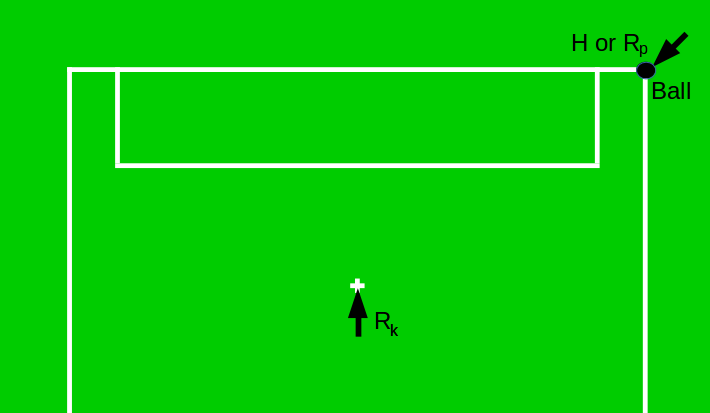
\includegraphics[width=0.6\textwidth]{img/tc_dynamic_kick.png}
\caption{\label{fig:tc_dynamic_kick}Setup for the moving ball challenge.}
\end{center}
\end{figure}

The initial setup of a run is presented in Fig.~\ref{fig:tc_dynamic_kick},
procedure is as follows:


\begin{enumerate}
\item The ball is placed on one corner of the field as chosen by the team taking the
technical challenge.
\item The robot $R_K$ is placed on the penalty mark.
\item The pass of the ball may either be performed by a human member from the
team $H$ or another robot, $R_P$. If the pass is performed by a robot, the team
may place $R_P$ after the referee has placed the ball. $R_p$ can be placed
anywhere on the field, at least 1m away from the ball.
\item The referee blows the whistle to start the run.
\item Teams may start the robot $R_P$ manually by pressing a button when the
run starts. But $R_K$ must not be touched after the referee blew the whistle. If
the pass is performed by a human, then the human is not allowed to wait before
kicking. Once the whistle is blown the human as 2 seconds to kick the ball,
otherwise the run is retaken.
\item A chronometer is started when $R_P$ or $H$ kicks the ball.
\end{enumerate}

{\bfseries Run evaluation}

\smallskip

The chronometer is stopped when the run ends. The causes for the end of a run and
the possible results are as following:
\begin{itemize}
\item \textit{Failure}
  \begin{itemize}
    \item The ball has been touched twice by $R_P$, $H$ or $R_K$.
    \item $R_k$ executed the kick motion but failed to kick the ball.
    \item The ball was kicked by $R_k$ but leaves the field without scoring a goal.
  \end{itemize}
\item \textit{Retake}
  \begin{itemize}
    \item The ball stops rolling or leaves the field before $R_k$ attempted to kick.
    \item The ball \emph{bounces} on $R_k$ rather than being kicked by $R_k$ and
          $R_k$ did not try to execute the kick motion before.
    \item The pass is performed by a human and the human did not kick 2 seconds after
          the whistle was blown.
  \end{itemize}
\item \textit{Partial success}
  \begin{itemize}
    \item Ball was kicked by $R_k$ but stopped rolling inside of the field.
  \end{itemize}
\item \textit{Success}
  \begin{itemize}
    \item Ball was kicked by $R_k$ and a goal was scored.
  \end{itemize}
\end{itemize}

{\bfseries Trials and ranking}

A trial consists of three different runs, each run ending with a \textit{Retake}
is restarted and do not count. A trial is considered as successful if at least 2
runs from the batch resulted in \textit{Success}. A trial is considered as
partially successful if at least 2 runs resulted in \textit{Success} or \textit{Partial success}.

The teams are ranked according to the following criteria on their best batch:
\begin{enumerate}
\item Number of \textit{Success} where the pass of the ball was executed by a robot
\item Number of \textit{Success} where the pass of the ball was executed by a human
\item Number of \textit{Partial success} where the pass of the ball was executed by a robot
\item Number of \textit{Partial success} where the pass of the ball was executed by a human
\item Average time for \textit{Success} runs, from first touch by $R_p$ or $H$ until goal is scored
\item Average shortest distance to the goal line for \textit{Partial success} runs
\end{enumerate}
